\subsection*{Problema 07}

\textbf{Enunciado:} 
Calcular la integral indefinida:
\begin{align*}
I = \int \dfrac{x \, dx}{x^2 - 4x + 4}
\end{align*}

\textbf{Solución:} 
Primero, analizamos el denominador de la función integrandia. Notamos que el trinomio cuadrado perfecto se puede factorizar de la siguiente manera:
\begin{align*}
x^2 - 4x + 4 = (x - 2)^2
\end{align*}

Sustituyendo esto en la integral dada, la expresión se reescribe como:
\begin{align*}
I = \int \dfrac{x}{(x - 2)^2} \, dx
\end{align*}

Para resolver esta integral, podemos utilizar el método de sustitución algebraica. Definimos una nueva variable $u$ tal que:
\begin{align*}
u &= x - 2 \\
du &= dx
\end{align*}

Además, despejamos la variable $x$ de la sustitución para expresarla en términos de $u$:
\begin{align*}
x = u + 2
\end{align*}

Sustituyendo $u$, $du$ y $x$ en la integral original, obtenemos:
\begin{align*}
I &= \int \dfrac{u + 2}{u^2} \, du
\end{align*}

Separamos la fracción en dos términos distintos para facilitar la integración:
\begin{align*}
I &= \int \left( \dfrac{u}{u^2} + \dfrac{2}{u^2} \right) du \\
I &= \int \left( \dfrac{1}{u} + 2u^{-2} \right) du
\end{align*}

Integramos cada término por separado aplicando las reglas básicas de integración:
\begin{align*}
I &= \int \dfrac{1}{u} \, du + \int 2u^{-2} \, du \\
I &= \ln|u| + 2 \left( \dfrac{u^{-1}}{-1} \right) + C \\
I &= \ln|u| - \dfrac{2}{u} + C
\end{align*}

Finalmente, regresamos a la variable original $x$ sustituyendo $u = x - 2$:
\begin{align*}
I = \ln|x - 2| - \dfrac{2}{x - 2} + C
\end{align*}

\begin{figure}[H]
	\centering
	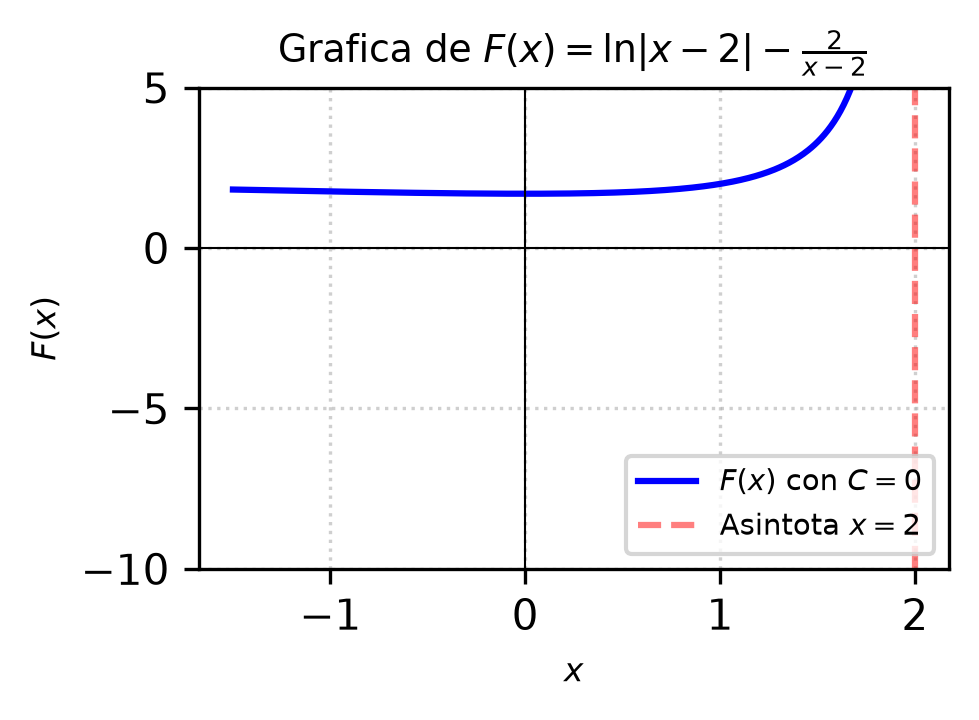
\includegraphics[width=\columnwidth]{semana_03/graficas/SEM03_P07_grafica.png}
	\caption{Representación gráfica de $f(x)$ y su antiderivada $F(x)$ evaluada para la constante de integración $C = 0$ (Problema 07).}
	\label{fig:problema07}
\end{figure}
